\chapter{Rezoluce v predikátové logice} 
\label{chapter:predicate-resolution}

V této kapitole si ukážeme, jak lze adaptovat rezoluční metodu, kterou jsme představili v Kapitole \ref{chapter:propositional-resolution}, na predikátovou logiku. Tato kapitola, poslední v části o predikátové logice, je poměrně rozsáhlá, proto uveďme přehled její struktury: 

\begin{itemize}
    \item Začneme neformálním úvodem (Sekce \ref{section:predicate-resolution-intro}).
\end{itemize}
V následujících třech sekcích představíme nástroje, které nám umožní vypořádat se se specifiky predikátové logiky: s kvantifikátory, proměnnými a termy.
\begin{itemize}
    \item V Sekci \ref{section:skolemization} si ukážeme, jak pomocí \emph{Skolemizace} odstranit kvantifikátory, abychom získali otevřené formule, které už lze převést do CNF.
    \item V Sekci \ref{section:grounding} vysvětlíme, že rezoluční zamítnutí bychom mohli hledat `na úrovni výrokové logiky' (tzv. \emph{grounding}), pokud bychom nejprve za proměnné substituovali `vhodné' konstantní termy.
    \item V Sekci \ref{section:unification} ukážeme, jak takové `vhodné' substituce hledat pomocí \emph{unifikačního algoritmu}.
\end{itemize}
Tím budeme mít všechny potřebné nástroje k představení vlastní rezoluční metody. Zbytek kapitoly má podobnou strukturu jako Kapitola \ref{chapter:propositional-resolution}.
\begin{itemize}
    \item Rezoluční pravidlo, rezoluční důkaz a související pojmy jsou popsány v Sekci \ref{section:predicate-resolution-method}.
    \item Sekce \ref{section:predicate-resolution-soundness-completeness} je věnována důkazu korektnosti a úplnosti.
    \item Na závěr, v Sekci \ref{section:predicate-LI-resolution}, popíšeme LI-rezoluci a její aplikaci v Prologu.
\end{itemize}


\section{Úvod}\label{section:predicate-resolution-intro}

Stejně jako ve výrokové logice, i v predikátové logice je rezoluční metoda založena na důkazu sporem. Chceme-li dokázat, že v teorii $T$ platí sentence $\varphi$ (tj. $T\models\varphi$), začneme s teorií $T\cup\{\neg \varphi\}$. Tuto teorii `převedeme' do CNF, a výslednou množinu klauzulí $S$ \emph{zamítneme} rezolucí (tj. ukážeme, že $S\proves_R\square$) čímž ukážeme, že je nesplnitelná.

Co myslíme konjunktivní normální formou? Roli \emph{literálu} hraje \emph{atomická formule}\footnote{Tj. $R(t_1,\dots,t_n)$ resp. $t_1=t_2$, kde $t_i$ jsou $L$-termy a $R$ je $n$-ární relační symbol z $L$.} nebo její negace. \emph{Klauzule} je (v množinové reprezentaci) konečná množina literálů, a \emph{formule} je množina klauzulí.\footnote{Jako ve výrokové logice připouštíme i nekonečné množiny klauzulí.} Jinak používáme stejnou terminologii, např. mluvíme o \emph{pozitivních}, \emph{negativních}, \emph{opačných} literálech, $\square$ značí prázdnou klauzuli (která je nesplnitelná), apod.

Nejprve si neformálně ukážeme specifika rezoluce v predikátové logice na několika velmi jednoduchých příkladech.

Všimněme si nejprve, že jsou-li teorie $T$ a sentence $\varphi$ \emph{otevřené} (neobsahují-li kvantifikátory), můžeme snadno sestrojit CNF formuli $S$ \emph{ekvivalentní} teorii $T\cup\{\neg \varphi\}$ (tj. mající stejnou množinu modelů). Nevadí ani univerzální kvantifikátory na začátku formule, ty můžeme odstranit beze změny významu.\footnote{Libovolná formule je ekvivalentní svému \emph{generálnímu uzávěru}, a ekvivalence platí oběma směry.}

\begin{example}
    Nechť $T=\{(\forall x)P(x),(\forall x)(P(x)\limplies Q(x))\}$ a $\varphi=(\exists x)Q(x)$. Je snadno vidět, že platí
    $$
    T\sim \{P(x),P(x)\limplies Q(x)\}\sim\{P(x),\neg P(x)\lor Q(x)\}
    $$ 
    a také:
    $$\neg\varphi=\neg(\exists x)Q(x)\sim(\forall x)\neg Q(x)\sim\neg Q(x)$$ 
    Teorii $T\cup\{\neg \varphi\}$ tedy můžeme převést na \emph{ekvivalentní} CNF formuli
    $$
    S = \{\{P(x)\},\{\neg P(x),Q(x)\},\{\neg Q(x)\}\}
    $$
    kterou snadno zamítneme rezolucí ve dvou krocích. (Představte si místo $P(x)$ výrokovou proměnnou $p$ a místo $Q(x)$ výrokovou proměnnou $q$.)
\end{example}

Obecně se nám to ale nepodaří, problémy dělá zejména existenční kvantifikátor. Na rozdíl od výrokové logiky \emph{není} každá teorie ekvivalentní CNF formuli. Ukážeme si ale postup, kterým lze vždy najít \emph{ekvisplnitelnou} CNF formuli, tj. takovou, která je nesplnitelná, \emph{právě když} $T\cup\{\neg \varphi\}$ je nesplnitelná, což nám k důkazu sporem stačí. Této konstrukci se říká \emph{Skolemizace} a spočívá v nahrazení existenčně kvantifikovaných proměnných nově přidanými konstantními resp. funkčními symboly. 

Například, formuli $(\exists x)\psi(x)$ nahradíme formulí $\psi(x/c)$, kde $c$ je nový konstantní symbol, který reprezentuje \emph{svědka}, tj. prvek, díky kterému je existenční kvantifikátor splněn. Protože takových prvků může být mnoho, ztrácíme \emph{ekvivalenci} teorií, platí ale, že je-li splnitelná původní formule, je splnitelná, i nová formule, a naopak.

\begin{example}
  Máme-li $T=\{(\exists x)P(x),P(x)\liff Q(x)\}$ a $\varphi=(\exists x)Q(x)$, potom 
  $$
  \neg\varphi\sim(\forall x)\neg Q(x)\sim\neg Q(x)
  $$
  a ekvivalenci můžeme převést do CNF jako obvykle, dostáváme:
  $$
  T\cup\{\neg \varphi\}\sim\{(\exists x)P(x),\neg P(x)\lor Q(x),\neg Q(x)\lor P(x),\neg Q(x)\}
  $$
  Formuli $(\exists x)P(x)$ nyní nahradíme $P(c)$, kde $c$ je nový konstantní symbol. Tím dostáváme CNF formuli:
  $$
  S = \{\{P(c)\},\{\neg P(x),Q(x)\},\{\neg Q(x),P(x)\},\{\neg Q(x)\}\}
  $$
  Ta není ekvivalentní teorii $T\cup\{\neg \varphi\}$, ale je s ní \emph{ekvisplnitelná} (v tomto případě jsou obě nesplnitelné).
\end{example}

Skolemizace může být i složitější, ne vždy stačí konstantní symbol. Pokud máme formuli tvaru $(\forall x)(\exists y)\psi(x,y)$, závisí zvolený svědek pro $y$ na zvolené hodnotě pro $x$, tedy `$y$ je funkcí $x$'. V tomto případě musíme $y$ nahradit $f(x)$, kde $f$ je nový unární funkční symbol. Tím dostáváme formuli $(\forall x)\psi(x,y/f(x))$ a univerzální kvantifikátor nyní můžeme odstranit a psát jen $\psi(x,y/f(x))$, což už je otevřená formule, byť v jiném jazyce (rozšířeném o symbol $f$). Skolemizaci formálně popíšeme, a potřebné vlastnosti dokážeme, v Sekci \ref{section:skolemization}. 

Nyní se podívejme na \emph{rezoluční pravidlo}. To je v predikátové logice složitější. Ukážeme si opět jen několik příkladů, formální definici necháme na později (Sekce \ref{section:predicate-resolution-method}).

\begin{example}
    V předchozím příkladu jsme dospěli k následující CNF formuli $S$, která je nesplnitelná, a chtěli bychom ji tedy rezolucí zamítnout:    
    $$
    S = \{\{P(c)\},\{\neg P(x),Q(x)\},\{\neg Q(x),P(x)\},\{\neg Q(x)\}\}
    $$
    Pokud bychom se na ni podívali `na úrovni výrokové logiky' (`ground level') a nahradili každou atomickou formuli novou výrokovou proměnnou, dostali bychom $\{\{r\},\{\neg p,q\},\{\neg q,p\},\{\neg q\}\}$, což není nesplnitelné. Potřebujeme využít toho, že $P(c)$ a $P(x)$ mají `podobnou strukturu' (jsou \emph{unifikovatelné}).

    Protože platí klauzule $\{\neg P(x),Q(x)\}$, platí i po provedení \emph{libovolné substituce}, tj. klauzule $\{\neg P(x/t),Q(x/t)\}$ je důsledkem $S$ pro libovolný term $t$. Mohli bychom si představit, že do  $S$ `přidáváme' všechny takto získané klauzule.\footnote{Těch je nekonečně mnoho, nekonečně mnoho je už jen \emph{variant} jedné klauzule, tj. klauzulí vzniklých pouhým přejmenováním proměnných. To nám ale nevadí, CNF formule může být dle definice nekonečná.} Výsledná CNF formule by po převedení na `úroveň výrokové logiky' už byla nesplnitelná. 
    
    \emph{Unifikační algoritmus} nám ale rovnou řekne, že správná substituce je $x/c$, a toto zahrneme už do \emph{rezolučního pravidla}, tedy \emph{rezolventou} klauzulí $\{P(c)\}$ a $\{\neg P(x),Q(x)\}$ bude klauzule $\{Q(c)\}$.
\end{example}

Unifikace může být i složitější, a upozorněme ještě na jeden rozdíl oproti výrokové logice: dovolíme si udělat rezoluci přes více literálů najednou, a to v případě, že jsou všechny dohromady \emph{unifikovatelné}:

\begin{example}
    Z klauzulí $\{R(x,f(x)),R(g(y),z)\}$ a $\{\neg R(g(c),u),P(u)\}$ (kde $R$ je binární relační, $f$ a $g$ jsou unární funkční, a $c$ konstantní symbol) bude možné odvodit rezolventu $\{P(f(g(c))\}$ za použití \emph{substituce} (\emph{unifikace}) $\{x/g(c),y/c,z/f(g(c)),u/f(g(c))\}$, kde z první klauzule vybíráme \emph{oba} literály najednou.
\end{example}

\begin{remark}
    To, že proměnné mají `lokální význam' v jednotlivých klauzulích (tj. můžeme za ně substituovat v jedné klauzuli aniž by to ovlivnilo ostatní klauzule), plyne z následující jednoduché tautologie, která platí pro libovolné formule $\psi,\chi$ (i pokud je v obou proměnná $x$ volná):
    $$
    \models(\forall x)(\psi \land \chi) \leftrightarrow (\forall x)\psi \land (\forall x)\chi
    $$
    
    Jak je vidět v předchozím příkladě, budeme také vyžadovat, aby klauzule v rezolučním pravidle měly disjunktní množiny proměnných; toho lze dosáhnout přejmenováním proměnných, což je speciální případ substituce.  
\end{remark}


\section{Skolemizace}\label{section:skolemization}

V této sekci ukážeme postup, jak redukovat otázku splnitelnosti dané teorie $T$ na otázku splnitelnosti \emph{otevřené} teorie $T'$. Připomeňme, že $T$ a $T'$ obecně nebudou ekvivalentní, budou ale \emph{ekvisplnitelné}:

\begin{definition}[Ekvisplnitelnost]
Mějme teorii $T$ v jazyce $L$ a teorii $T'$ v ne nutně stejném jazyce $L'$. Říkáme, že $T$ a $T'$ jsou \emph{ekvisplnitelné}, 
pokud platí: 
$$
\text{$T$ má model}\ \Leftrightarrow\ \text{$T'$ má model}
$$
\end{definition}

Celá konstrukce sestává z následujících kroků, které vysvětlíme níže:
\begin{enumerate}
    \item Převod do \emph{prenexní normální formy} (vytýkání kvantifikátorů).
    \item Nahrazení formulí jejich generálními uzávěry (abychom získali sentence).
    \item Odstranění existenčních kvantifikátorů (nahrazení sentencí \emph{Skolemovými variantami}).
    \item Odstranění zbývajících univerzálních kvantifikátorů (výsledkem jsou otevřené formule).
\end{enumerate}

\subsection{Prenexní normální forma}

Nejprve ukážeme postup, jakým můžeme z libovolné formule `vytknout' kvantifikátory, tj. převést do tzv. \emph{prenexní normální formy}, která začíná posloupností kvantifikátorů, a pokračuje už jen volnou formulí.

\begin{definition}[PNF]
    Formule $\varphi$ je v \emph{prenexní normální formě (PNF)}, je-li tvaru
    $$
    (Q_1x_1)\dots(Q_nx_n)\varphi'
    $$
    kde $Q_i$ je kvantifikátor ($\forall$ nebo $\exists$) a formule $\varphi'$ je otevřená. Formuli $\varphi'$ potom říkáme \emph{otevřené jádro} $\varphi$ a $(Q_1x_1)\dots(Q_nx_n)$ je \emph{kvantifikátorový prefix}. 
    
    Je-li $\varphi$ formule v PNF a jsou-li všechny kvantifikátory univerzální, potom říkáme, že $\varphi$ je \emph{univerzální} formule.
\end{definition}

Cílem této podsekce je ukázat následující tvrzení:

\begin{proposition}[Převod do PNF]\label{proposition:convert-to-pnf}
    Ke každé formuli $\varphi$ existuje ekvivalentní formule v prenexní normální formě.    
\end{proposition}

Algoritmus bude podobně jako převod do CNF založen na nahrazování podformulí \emph{ekvivalentními} podformulemi, s cílem posunout kvantifikátory blíže ke kořeni stromu formule. Co myslíme ekvivalencí formulí $\varphi\sim\varphi'$? To, že mají stejný význam, tj. v každém modelu a při každém ohodnocení proměnných mají touž pravdivostní hodnotu. Ekvivalentně, že platí $\models\varphi\liff\varphi'$. Budeme potřebovat následující jednoduché pozorování:

\begin{observation}\label{observation:pnf-one-step}
    Nahradíme-li ve formuli $\varphi$ nějakou podformuli $\psi$ ekvivalentní formulí $\psi'$, potom je i výsledná formule $\varphi'$ ekvivalentní formuli $\varphi$.
\end{observation}

Převod je založen na opakovaném použití následujících syntaktických pravidel:

\begin{lemma}\label{lemma:pnf-conversion-rules}
    Označme jako $\overline{Q}$ kvantifikátor opačný ke $Q$. Nechť $\varphi$ a $\psi$ jsou formule, a proměnná $x$ nechť není volná ve formuli $\psi$. Potom platí:
    \begin{align*}
        \neg (Qx)\varphi\ &\sim\ (\overline{Q}x)\neg\varphi\\
        (Qx)\varphi \land \psi\ &\sim\ (Qx)(\varphi \land \psi)\\
        (Qx)\varphi \lor \psi\ &\sim\ (Qx)(\varphi \lor \psi)\\
        (Qx)\varphi \limplies \psi\ &\sim\ (\overline{Q}x)(\varphi \limplies \psi)\\
        \psi \limplies (Qx)\varphi\ &\sim\ (Qx)(\psi \limplies \varphi)
    \end{align*}
\end{lemma}
\begin{proof}
    Pravidla lze snadno ověřit sémanticky, nebo dokázat tablo metodou (v tom případě nejde-li o sentence, musíme je nahradit jejich generálními uzávěry).   
\end{proof}

Všimněte si, že v pravidle $(Qx)\varphi \limplies \psi\sim(\overline{Q}x)(\varphi \limplies \psi)$ pro vytýkání z \emph{antecendentu} implikace musíme změnit kvantifikátor (z $\forall$ na $\exists$ a naopak) zatímco při vytýkání z \emph{konsekventu} zůstává kvantifikátor stejný. Proč tomu tak je vidíme nejlépe pokud přepíšeme implikaci pomocí disjunkce a negace:
$$
(Qx)\varphi \limplies \psi\sim\neg(Qx)\varphi \lor\psi\sim(\overline{Q}x)(\neg\varphi)\lor\psi\sim(\overline{Q}x)(\neg\varphi\lor\psi)\sim (\overline{Q}x)(\varphi \limplies \psi)
$$
Všimněte si také předpokladu, že $x$ není volná v $\psi$. Bez něj by pravidla nefungovala, viz např:
$$
(\exists x)P(x)\land Q(x)\ \not\sim\ (\exists x)(P(x)\land Q(x))
$$
V takové situaci nahradíme formuli variantou, ve které přejmenujeme vázanou proměnnou $x$ na nějakou novou proměnnou: 
$$
(\exists x)P(x)\land Q(x)\ \sim\ (\exists y)P(y)\land Q(x) \sim (\exists y)(P(y)\land Q(x))
$$
\begin{exercise}
    Dokažte Pozorování \ref{observation:pnf-one-step} a všechna pravidla z Lemmatu \ref{lemma:pnf-conversion-rules}.
\end{exercise}

Ukažme si postup na jednom příkladě:

\begin{example}\label{example:convert-to-pnf}
    Převeďme formuli $((\forall z)P(x,z)\land P(y,z))\ \limplies\ \neg(\exists x)P(x,y)$ do PNF. Zapíšeme jen jednotlivé mezikroky. Všimněte si, jaké pravidlo na jakou podformuli bylo použito (a také přejmenování proměnné v prvním kroku), a sledujte postup na stromu formule.
    \begin{align*}
        &\ (\forall z)P(x,z)\land P(y,z)\ \limplies\ \neg(\exists x)P(x,y)\\ \sim &\ 
        (\forall u) P(x,u)\land P(y,z)\ \limplies\ (\forall x)\neg P(x,y)\\ \sim &\ 
        (\forall u)(P(x,u)\land P(y,z))\ \limplies\ (\forall v)\neg P(v,y)\\ \sim &\ 
        (\exists u)( P(x,u)\land P(y,z)\ \limplies\ (\forall v)\neg P(v,y))\\ \sim &\ 
        (\exists u)(\forall v)( P(x,u)\land P(y,z)\ \limplies\ \neg P(v,y))
        \end{align*}    
\end{example}

Nyní nám již nic nebrání dokázat Tvrzení \ref{proposition:convert-to-pnf}:

\begin{proof}[Důkaz Tvrzení \ref{proposition:convert-to-pnf}]
    Indukcí podle struktury formule $\varphi$ s využitím Lemmatu \ref{lemma:pnf-conversion-rules} a Pozorování \ref{observation:pnf-one-step}.
\end{proof}

Protože je každá formule $\varphi(x_1,\dots,x_n)$ ekvivalentní svému \emph{generálnímu uzávěru} $$(\forall x_1)\dots(\forall x_n)\varphi(x_1,\dots,x_n)$$ můžeme Tvrzení \ref{proposition:convert-to-pnf} vyslovit také takto:

\begin{corollary}
    Ke každé formuli $\varphi$ existuje ekvivalentní \emph{sentence} v PNF.
\end{corollary} 

Například v Příkladě \ref{example:convert-to-pnf} je výsledná sentence $(\forall x)(\forall y)(\forall z)(\exists u)(\forall v)( P(x,u)\land P(y,z)\limplies\neg P(v,y))$.

\begin{remark}
    Prenexní forma není jednoznačná, pravidla pro převod můžeme aplikovat v různém pořadí. Jak uvidíme v následující podsekci, je výhodné vytýkat přednostně kvantifikátory [ze kterých se stanou] existenční: Máme-li na výběr mezi $(\forall x)(\exists y)\varphi(x,y)$ a $(\exists y)(\forall x)\varphi(x,y)$, volíme druhou variantu, neboť v první je `$y$ závislé na $x$'.
\end{remark}



\subsection{Skolemova varianta}

Nyní jsme převedli naše axiomy na ekvivalentní sentence v prenexním tvaru. Pokud by některá sentence obsahovala pouze univerzální kvantifikátory, tj. byla tvaru 
$$(\forall x_1)\dots(\forall x_n)\varphi(x_1,\dots,x_n)$$ 
kde $\varphi$ je otevřená, mohli bychom ji prostě nahradit jejím otevřeným jádrem $\varphi$, které je jí v tomto případě ekvivalentní. Jak si ale poradit s existenčními kvantifikátory, např. $(\exists x)\varphi(x)$, $(\forall x)(\exists y)\varphi(x,y)$, apod? Ty nejprve nahradíme jejich \emph{Skolemovou variantou}.

\begin{definition}[Skolemova varianta]
Mějme $L$-sentenci $\varphi$ v PNF, a nechť všechny její vázané proměnné jsou různé. Nechť existenční kvantifikátory z prefixu $\varphi$ jsou $(\exists y_1),\dots,(\exists y_n)$ (v tomto pořadí), a nechť pro každé $i$ jsou $(\forall x_1),\dots,(\forall x_{n_i})$ právě všechny univerzální kvantifikátory předcházející kvantifikátor $(\exists y_i)$ v prefixu $\varphi$. 

Označme $L'$ rozšíření $L$ o \emph{nové} $n_i$-ární funkční symboly $f_1,\dots,f_n$, kde symbol $f_i$ je arity $n_i$, pro každé $i$. \emph{Skolemova varianta} sentence $\varphi$ je $L'$-sentence $\varphi_S$ vzniklá z $\varphi$ tak, že pro každé $i=1,\dots,n$:
\begin{itemize}
    \item odstraníme z prefixu kvantifikátor $(\exists y_i)$, a
    \item substituujeme za proměnnou $y_i$ term $f_i(x_1,\dots,x_{n_i})$.
\end{itemize}
Tomuto procesu říkáme také \emph{skolemizace}.
\end{definition}

\begin{example}
    Skolemova varianta sentence 
    $$\varphi=(\exists y_1)(\forall x_1)(\forall x_2)(\exists y_2)(\forall x_3)R(y_1,x_1,x_2,y_2,x_3)$$
    je sentence
    $$
    \varphi_S=(\forall x_1)(\forall x_2)(\forall x_3)R(f_1,x_1,x_2,f_2(x_1,x_2),x_3)
    $$
    kde $f_1$ je nový konstantní symbol a $f_2$ je nový binární funkční symbol.
\end{example}

\begin{remark}
    Nezapomeňte, že při skolemizaci musíme vycházet ze sentence! Například, máme-li formuli $(\exists y)E(x,y)$, není $E(x,c)$ její Skolemova varianta. Musíme napřed provést generální uzávěr $(\forall x)(\exists y)E(x,y)$, a potom správně skolemizovat jako $(\forall x)E(x,f(x))$, což je ekvivalentní otevřené formuli $E(x,f(x))$ (která říká něco mnohem slabšího než $E(x,c)$).

    Je také důležité, aby každý symbol použitý při skolemizaci byl opravdu nový, jeho jedinou `rolí' v celé teorii musí být reprezentovat `existující' prvky v této formuli.
\end{remark} 

V následujícím lemmatu ukážeme klíčovou vlastnost skolemovy varianty:

\begin{lemma}\label{lemma:skolem-variant-conservative-extension}
Mějme $L$-sentenci $\varphi=(\forall x_1)\dots(\forall x_n)(\exists y)\psi$ a nechť $\varphi'$ je sentence 
$$
(\forall x_1)\dots(\forall x_n)\psi(y/f(x_1,\dots,x_n))$$
kde $f$ je nový funkční symbol. Potom:
\begin{enumerate}[(i)]
    \item $L$-redukt každého modelu $\varphi'$ je modelem $\varphi$, a 
    \item každý model $\varphi$ lze expandovat na model $\varphi'$.
\end{enumerate}
\end{lemma}

\begin{proof}
    Nejprve dokažme část (i): Mějme model $\A'\models\varphi'$ a nechť $\A$ je jeho redukt na jazyk $L$. Pro každé ohodnocení proměnných $e$ platí $\A\models\psi[e(y/a)]$ pro $a=(f(x_1,\dots,x_n))^{\A'}[e]$, tedy $\A\models\varphi$.
    
    Nyní část (ii): Protože $\A\models\varphi$, existuje funkce $f^A:A^n\to A$ taková, že pro každé ohodnocení proměnných $e$ platí $\A\models \psi[e(y/a)]$, kde $a=f^A(e(x_1),\dots,e(x_n))$. To znamená, že expanze struktury $\A$ vzniklá přidáním funkce $f^A$ je modelem $\varphi'$.    
\end{proof}

\begin{remark}
    Expanze modelu ve druhé části tvrzení nemusí být (a typicky není) jednoznačná, na rozdíl od extenze o definici nového funkčního symbolu.
\end{remark}

Aplikujeme-li předchozí lemma opakovaně (postupně pro všechny existenční kvantifikátory), získáme následující důsledek:

\begin{corollary}
    Sentence $\varphi$ a její skolemova varianta $\varphi_S$ jsou ekvisplnitelné.
\end{corollary}


\subsection{Skolemova věta}

V této podsekci shrneme celý postup popsaný v předchozích podsekcích. Klíčem je následující věta norského logika Thoralfa Skolema:

\begin{theorem}[Skolemova věta]
    Každá teorie má otevřenou konzervativní extenzi.
\end{theorem}
\begin{proof}
    Mějme $L$-teorii $T$. Každý axiom nahradíme jeho generálním uzávěrem (není-li to už sentence) a převedeme do PNF, tím získáme ekvivalentní teorii $T'$. Nyní nahradíme každý axiom teorie $T'$ jeho Skolemovou variantou. Tím získáme teorii $T''$ v rozšířeném jazyce $L'$. Z Lemmatu \ref{lemma:skolem-variant-conservative-extension} plyne, že $L$-redukt každého modelu $T''$ je modelem $T'$, tedy $T''$ je extenzí $T'$, a že každý model $T'$ lze expandovat do jazyka $L'$ na model $T''$, tedy jde o konzervativní extenzi. Teorie $T''$ je axiomatizovaná univerzálními sentencemi, odstraníme-li kvantifikátorové prefixy (tj. vezmeme-li jádra axiomů), získáme otevřenou teorii $T'''$, která ekvivalentní s $T''$ a tedy je také konzervativní extenzí $T$.
\end{proof}

Ze sémantické charakterizace konzervativní extenze snadno plyne následující důsledek:

\begin{corollary}
    Ke každé teorii můžeme pomocí skolemizace najít ekvisplnitelnou otevřenou teorii.
\end{corollary}

Otevřenou teorii už můžeme snadno převést do CNF (vyjádřit \emph{formulí} $S$ v množinové reprezentaci) pomocí ekvivalentních syntaktických úprav, stejně jako ve výrokové logice (viz Sekce \ref{subsection:convert-to-normal-form}).


\section{Grounding}\label{section:grounding}

V této sekci si ukážeme, že máme-li otevřenou teorii, která je nesplnitelná, můžeme její nesplnitelnost doložit `na konkrétních prvcích'. Co tím myslíme? Existuje konečně mnoho \emph{základních (ground) instancí} axiomů (instancí, kde za proměnné substituujeme konstantní termy), takových, že jejich konjunkce (která neobsahuje žádnou proměnnou) je nesplnitelná. 

\begin{definition}[Základní instance]
    Mějme otevřenou formuli $\varphi$ ve volných proměnných $x_1,\dots,x_n$. Řekneme, že instance $\varphi(x_1/t_1,\dots,x_n/t_n)$ je \emph{základní (ground) instance}, jsou-li všechny termy $t_1,\dots,t_n$ konstantní (ground).
\end{definition}

\begin{example}
    Teorie $T=\{P(x,y)\lor R(x,y),\neg P(c,y),\neg R(x,f(x))\}$ v jazyce $L=\langle P,R,f,c \rangle$ nemá model. Můžeme to doložit následující konjunkcí základních instancí axiomů, kde za proměnnou $x$ substituujeme konstantu $c$ a za $y$ konstantní term $f(c)$:
$$
(P(c,f(c))\lor R(c,f(c)))\ \land\ \neg P(c,f(c))\ \land\ \neg R(c,f(c))
$$
\end{example}
Tato sentence je zjevně nesplnitelná. Základní atomické sentence $(P(c,f(c))$ a $R(c,f(c))$ můžeme navíc (díky tomu, že neobsahují proměnné) chápat jako výrokové proměnné $p_1,p_2$, kde $p_1$ znamená `platí $P(c,f(c))$' a $p_2$ znamená `platí $R(c,f(c))$'. Dostáváme potom následující výrok, který lze snadno zamítnout rezolucí:
$$
(p_1 \lor p_2) \land \neg p_1 \land \neg p_2
$$
Tomuto procesu převedení na základní instance (a tím do výrokové logiky) říkáme `grounding'. Za chvíli ho zformalizujeme a dokážeme \emph{Herbrandovu větu},\footnote{Francouzský matematik Jacques Herbrand pracoval na konci 20. let 20. století. Během své krátké kariéry (zemřel tragicky ve věku 23 let) objevil několik dalších důležitých výsledků, a mimo jiné formalizoval pojem rekurzivní funkce.} která říká, že taková nesplnitelná konjunkce základních instancí axiomů existuje pro každou nesplnitelnou teorii.

\subsection{Přímá redukce do výrokové logiky}

Uvědomme si nyní, že díky Herbrandově větě grounding umožňuje následující postup, byť neefektivní, jak zamítat formule rezolucí `na úrovni výrokové logiky': Ve vstupní formuli $S$ nahradíme každou klauzuli množinou všech jejích základních instancí (pokud žádné nejsou, tedy pokud jazyk neobsahuje konstantní symbol, jeden konstantní symbol do jazyka přidáme). Ve výsledné množině klauzulí $S'$ chápeme atomické sentence jako výrokové proměnné, a $S'$ zamítneme výrokovou rezolucí (o které víme, že je korektní a úplná). 

Problémem tohoto přístupu je, že klauzulí v $S'$ (základních instancí klauzulí z $S$) může být mnoho, i nekonečně mnoho, např. kdykoliv je v jazyce alespoň jeden funkční (nekonstantní) symbol. 

\begin{example}
Máme-li CNF formuli $S=\{\{P(x,y),R(x,y)\},\{\neg P(c,y)\},\{\neg R(x,f(x))\}\}$ v jazyce $L=\langle f,c\rangle$, nahradíme ji následující nekonečnou formulí $S'$:
\begin{align*}
    S'=\{&\{P(c,c),R(c,c)\},\{P(c,f(c)),R(c,f(c))\},\{P(f(c),c),R(f(c),c)\},\dots,\\ 
    &\{\neg P(c,c)\}, \{\neg P(c,f(c))\},\{\neg P(c,f(f(c)))\},\{\neg P(c,f(f(f(c))))\}, \dots,\\
    &\{\neg R(c,f(c))\}, \{\neg R(f(c),f(f(c)))\},\{\neg R(f(f(c)),f(f(f(c))))\},\dots\}    
\end{align*}
Ta je nesplnitelná, neboť obsahuje následující konečnou podmnožinu, která je nesplnitelná, což snadno ukážeme výrokovou rezolucí:
$$
\{\{P(c,f(c)),R(c,f(c))\},\{\neg P(c,f(c))\},\{\neg R(c,f(c))\}\}\proves_R\square
$$
\end{example}
V Sekci \ref{section:unification} si ukážeme efektivní postup jak hledat vhodné základní instance klauzulí, pomocí tzv. \emph{unifikace}.


\subsection{Herbrandova věta}

V této podsekci vyslovíme a dokážeme Herbrandovu větu. Budeme předpokládat, že jazyk obsahuje nějaký konstantní symbol: pokud v jazyce žádný není, jeden přidáme. Konstantní symbol potřebujeme k tomu, aby existovaly konstantní termy, a my mohli vytvořit tzv. \emph{Herbrandův model}. Jde o konstrukci sémantického objektu (modelu) ze syntaktických objektů (konstantních termů) velmi podobnou \emph{kanonickému modelu} (Definice \ref{definition:canonical-model-predicate}).\footnote{Rozdíl je v tom, že nepřidáváme spočetně mnoho nových konstantních symbolů (vycházíme jen z konstantních symbolů, které už v jazyce jsou), a také nijak nepředepisujeme, jak mají vypadat relace modelu.}

\begin{definition}[Herbrandův model]
Mějme jazyk $L=\langle\mathcal R,\mathcal F\rangle$ s alespoň jedním konstantním symbolem. $L$-struktura $\A=\langle A,\mathcal R^\A,\mathcal F^\A\rangle$ je \emph{Herbrandův model}, jestliže:
\begin{itemize}
    \item $A$ je množina všech konstantních $L$-termů (tzv. \emph{Herbrandovo univerzum}), a
    \item pro každý $n$-ární funkční symbol $f\in\mathcal F$ a konstantní termy $\text{``$t_1$''},\dots,\text{``$t_n$''}\in A$ platí:
    $$
    f^\A(\text{``$t_1$''},\dots,\text{``$t_n$''})=\text{``$f(t_1,\dots,t_n)$''}
    $$
    \item Speciálně, pro každý konstantní symbol $c\in\mathcal F$ je $c^\A=\text{``$c$''}$.
\end{itemize}
Na interpretace relačních symbolů neklademe žádné podmínky.
\end{definition}

Připomeňme, že uvozovky okolo termů píšeme jen neformálně, abychom jasněji odlišili termy jako syntaktické objekty (řetězce symbolů) od jejich interpretací (funkcí).

\begin{example}
Mějme jazyk $L=\langle P,f,c\rangle$, kde $P$ je unární relační, $f$ je binární funkční, a $c$ konstantní symbol. Herbrandovo univerzum pro tento jazyk je množina
$$
A=\{\text{``$c$''},\text{``$f(c,c)$''},\text{``$f(c,f(c,c))$''},\text{``$f(f(c,c),c)$''}\dots\}
$$
Struktura $\A=\langle A,P^\A,f^\A,c^\A\rangle$ je Herbrandův model, jestliže $c^\A=\text{``$c$''}$ a funkce $f^\A$ splňuje:
\begin{itemize}
    \item $f^\A(\text{``$c$''},\text{``$c$''})=\text{``$f(c,c)$''}$,
    \item $f^\A(\text{``$c$''},\text{``$f(c,c)$''})=\text{``$f(c,f(c,c))$''}$,
    \item $f^\A(\text{``$f(c,c)$''},\text{``$c$''})=\text{``$f(f(c,c),c)$''}$, atd.
\end{itemize}
Relace $P^\A$ může být libovolná podmnožina $A$.
\end{example}

Nyní jsme připraveni vyslovit Herbrandovu větu. Neformálně řečeno, je-li teorie splnitelná, tj. má-li model, potom má dokonce Herbrandův model, a v opačném případě najdeme nesplnitelnou konjunkci základních instancí axiomů, použitelnou pro rezoluční zamítnutí `na úrovni výrokové logiky'.


\begin{theorem}[Herbrandova věta]
Mějme otevřenou teorii $T$ v jazyce $L$ bez rovnosti a s alespoň jedním konstantním symbolem. Potom buď má $T$ \emph{Herbrandův model}, nebo existuje konečně mnoho základních instancí axiomů $T$, jejichž konjunkce je nesplnitelná.
\end{theorem}
\begin{proof}
Označme jako $T_\text{ground}$ množinu všech základních instancí axiomů teorie $T$. Zkonstruujeme systematické\footnote{Nebo libovolné dokončené tablo, ale tak, abychom sporné větve už neprodlužovali.} tablo z teorie $T_\text{ground}$ s položkou $\F\bot$ v kořeni, ale z jazyka $L$, bez rozšíření o pomocné konstantní symboly na jazyk $L_C$.\footnote{Protože v $T_\text{ground}$ nejsou žádné kvantifikátory, pomocné symboly nikde v tablu nejsou použity.}

Pokud tablo obsahuje bezespornou větev, potom je kanonický model pro tuto větev (opět bez přidání pomocných konstantních symbolů) Herbrandovým modelem $T$. V opačném případě máme tablo důkaz sporu, tedy teorie $T_\text{ground}$, a tím pádem i $T$, je nesplnitelná. Protože je tablo důkaz konečný, použili jsme v něm jen konečně mnoho základních instancí axiomů $\alpha_\text{ground}\in T_\text{ground}$. Jejich konjunkce je tedy nesplnitelná.
\end{proof}

\begin{remark}
Máme-li jazyk s rovností, potom nejprve teorii $T$ rozšíříme o axiomy rovnosti na teorii $T^*$, a má-li $T^*$ Herbrandův model $\A$, faktorizujeme ho podle kongruence $=^A$, stejně jako v případě kanonického modelu.
\end{remark}

Na závěr této sekce vyslovíme dva důsledky Herbrandovy věty.

\begin{corollary}
    Mějme otevřenou formuli $\varphi(x_1,\dots,x_n)$ v jazyce $L$ s alespoň jedním konstantním symbolem. Potom existují konstantní $L$-termy $t_{ij}$ ($1\leq i\leq m,1\leq j\leq n$) takové, že sentence 
    $$
    (\exists x_1)\dots(\exists x_n)\varphi(x_1,\dots,x_n)$$ 
    je pravdivá, právě když je následující formule (výroková) tautologie:
    $$
    \varphi(x_1/t_{11},\dots,x_n/t_{1n})\lor \dots \lor \varphi(x_1/t_{m1},\dots,x_n/t_{mn})
    $$
\end{corollary}
\begin{proof}
Sentence $(\exists x_1)\dots(\exists x_n)\varphi(x_1,\dots,x_n)$ je pravdivá, právě když $(\forall x_1)\dots(\forall x_n)\neg\varphi$ je nesplnitelná, neboli když $\neg\varphi$ je nesplnitelná. Tvrzení plyne z Herbrandovy věty aplikované na teorii $T=\{\neg\varphi\}$.
\end{proof}

\begin{corollary}\label{corollary:herbrands-theorem-corollary-ground}
    Mějme otevřenou teorii $T$ v jazyce s alespoň jedním konstantním symbolem. Teorie $T$ má model, právě když má model teorie $T_\text{ground}$ sestávající ze všech základních instancí axiomů teorie $T$.
\end{corollary}
\begin{proof}
V modelu teorie $T$ platí všechny axiomy, tedy i všechny základní instance axiomů. Je tedy i modelem $T_\text{ground}$. Pokud $T$ nemá model, podle Herbrandovy věty je nějaká konečná podmnožina teorie $T_\text{ground}$ nesplnitelná.
\end{proof}


\section{Unifikace}\label{section:unification}

Místo substitucí \emph{všech} základních termů a práce s touto novou, obrovskou a typicky nekonečnou množinou klauzulí, je lepší najít v konkrétním rezolučním kroku `vhodnou' substituci a pracovat jen s ní. V této sekci vysvětlíme, co znamená `vhodná' (tzv. \emph{unifikace}) a jak ji lze hledat (pomocí \emph{unifikačního 
algoritmu}).

\subsection{Substituce}
%\todo change terms of sigma to s and tau to t?

Nejprve uveďme několik příkladů `vhodných' substitucí:

\begin{example}\label{example:substitutions}
\begin{itemize}
    \item Z klauzulí $\{P(x),Q(x,a)\}$ a $\{\neg P(y),\neg Q(b,y)\}$ získáme pomocí substituce $\{x/b,y/a\}$ klauzule $\{P(b),Q(b,a)\}$ a $\{\neg P(a),\neg Q(b,a)\}$, a z nich potom rezolucí klauzuli $\{P(b),\neg P(a)\}$. Mohli bychom také použít substituci $\{x/y\}$ a rezolucí přes $P(y)$ získat rezolventu $\{Q(y,a),\neg Q(b,y)\}$.
    \item Máme-li klauzule $\{P(x),Q(x,a),Q(b,y)\}$ a $\{\neg P(v),\neg Q(u,v)\}$, vhodnou substitucí je $\{x/b,y/a,u/b,v/a\}$; dostáváme $\{P(b),Q(b,a)\}$ a $\{\neg P(a),\neg Q(b,a)\}$, jejichž rezolventou je $\{P(b),\neg P(a)\}$.
    \item Podívejme se ještě na klauzule $\{P(x),Q(x,z)\}$ a $\{\neg P(y),\neg Q(f(y),y)\}$. Mohli bychom použít substituci $\{x/f(a),y/a,z/a\}$ a získat tak dvojici klauzulí $\{P(f(a)),Q(f(a),a)\}$ a $\{\neg P(a),\neg Q(f(a),a)\}$, rezolucí potom $\{P(f(a)),\neg P(a)\}$.
    
    Lepší ale bude využít substituce $\{x/f(z),y/z\}$, po které máme $\{P(f(z)),Q(f(z),z)\}$ a $\{\neg P(z),\neg Q(f(z),z)\}$, a rezolventu $\{P(f(z)),\neg P(z)\}$. Tato substituce je \emph{obecnější}, a výsledná rezolventa `říká více' než $\{P(f(a)),\neg P(a)\}$ (ta je jejím důsledkem, ale naopak to neplatí).
\end{itemize}
\end{example}

Nyní zavedeme potřebnou terminologii týkající se substitucí. Substituce budeme aplikovat na termy nebo na literály (atomické formule nebo jejich negace), označme tyto dohromady jako \emph{výrazy}. 

\begin{definition}[Substituce]
    \emph{Substituce} je konečná množina $\sigma=\{x_1/t_1,\dots,x_n/t_n\}$, kde $x_i$ jsou navzájem různé proměnné a $t_i$ jsou termy, přičemž vyžadujeme, aby term $t_i$ nebyl roven proměnné $x_i$. Substituce $\sigma$ je 
    \begin{itemize}
        \item \emph{základní}, jsou-li všechny termy $t_i$ konstantní,
        \item \emph{přejmenování proměnných}, jsou-li všechny termy $t_i$ navzájem různé proměnné.
    \end{itemize}
    \emph{Instance} výrazu (termu nebo literálu) $E$ \emph{při substituci $\sigma=\{x_1/t_1,\dots,x_n/t_n\}$} je výraz vzniklý z $E$ simultánním nahrazením všech výskytů proměnných $x_i$ termy $t_i$, označme jej $E\sigma$. Je-li $S$ množina výrazů, potom značíme $S\sigma=\{E\sigma\mid E\in S\}$.
\end{definition}

Protože proměnné nahrazujeme \emph{simultánně} pro všechny proměnné zároveň, případný výskyt proměnné $x_i$ v termu $t_j$ nepovede ke zřetězení substitucí.

\begin{example}
Například pro $S=\{P(x),R(y,z)\}$ a substituci $\sigma=\{x/f(y,z),y/x,z/c\}$ máme:
$$
S\sigma=\{P(f(y,z)),R(x,c)\}
$$
\end{example}

Substituce můžeme přirozeně \emph{skládat}. Složení substitucí $\sigma$ a $\tau$, kde nejprve aplikujeme $\sigma$ a potom~$\tau$, budeme zapisovat jako $\sigma\tau$. Bude tedy platit $E(\sigma\tau)=(E\sigma)\tau$, pro libovolný výraz~$E$.

\begin{example}\label{example:compose-substitutions}
    Začněme opět příkladem. Máme-li výraz $E=P(x,w,u)$, a substituce \begin{align*}
        \sigma&=\{x/f(y),w/v\}\\
        \tau&=\{x/a,y/g(x),v/w,u/c\}
    \end{align*}
    potom je $E\sigma=P(f(y),v,u)$ a $(E\sigma)\tau=P(f(g(x)),w,c)$.
    Musí tedy platit: 
    $$
    \sigma\tau=\{x/f(g(x)),y/g(x),v/w,u/c\}
    $$
\end{example}

Nyní formální definice:

\begin{definition}[Skládání substitucí]
Mějme substituce $\sigma=\{x_1/t_1,\dots,x_n/t_n\}$ a $\tau=\{y_1/s_1,\dots,y_m/s_m\}$. \emph{Složení substitucí $\sigma$ a $\tau$} je substituce
$$
\sigma\tau=\{x_i/t_i\tau\mid x_i\in X,x_i\neq t_i\tau\}\cup\{y_j/s_j\mid y_j\in Y\setminus X\}
$$
kde $X=\{x_1,\dots,x_n\}$ a $Y=\{y_1,\dots,y_m\}$.
\end{definition}

Všimněte si, že skládání substitucí není komutativní, $\sigma\tau$ je typicky zcela jiná substituce než $\tau\sigma$.

\begin{example}
    Jsou-li $\sigma$ a $\tau$ jako v Příkladu \ref{example:compose-substitutions}, potom: 
    $$
    \tau\sigma=\{x/a,y/g(f(y)),u/c,w/v\}\neq \sigma\tau
    $$
\end{example}

Nyní ukážeme, že takto definované skládání substitucí splňuje požadovanou vlastnosti, a také že je \emph{asociativní}. Z asociativity plyne, že nemusíme (a také nebudeme) psát závorky ve složení $\sigma\tau\varrho$, $\sigma_1\sigma_2\cdots\sigma_n$ apod.

\begin{proposition}
Mějme substituce $\sigma$, $\tau$, $\varrho$, a libovolný výraz $E$. Potom platí:
\begin{enumerate}[(i)]
    \item $(E\sigma)\tau=E(\sigma\tau)$
    \item $(\sigma\tau)\varrho=\sigma(\tau\varrho)$
\end{enumerate}
\end{proposition}

\begin{proof}
Nechť $\sigma=\{x_1/t_1,\dots,x_n/t_n\}$ a $\tau=\{y_1/s_1,\dots,y_m/s_m\}$. Stačí dokázat v případě, kdy výraz $E$ je jediná proměnná, zbytek snadno plyne indukcí. (Substituce nijak nemění ostatní symboly.) Rozdělíme na tři případy:
\begin{itemize}
    \item Je-li $E=x_i$ pro nějaké $i$, potom $E\sigma=t_i$ a $(E\sigma)\tau=t_i\tau=E(\sigma\tau)$, kde druhá rovnost je z definice $\sigma\tau$.
    \item Je-li $E=y_j$ pro nějaké $j$, kde $y_j\notin\{x_1,\dots,x_n\}$, potom $E\sigma=E$ a $(E\sigma)\tau=E\tau=s_j=E(\sigma\tau)$ opět z definice $\sigma\tau$.
    \item Je-li $E$ jiná proměnná, potom $(E\sigma)\tau=E=E(\sigma\tau)$.
\end{itemize}
Tím jsme dokázali (i). Asociativitu (ii) snadno dokážeme opakovaným užitím (i). Následující platí pro každý výraz $E$, tedy i pro každou proměnnou:
$$
E((\sigma\tau)\varrho)=(E(\sigma\tau))\varrho=((E\sigma)\tau)\varrho=(E\sigma)(\tau\varrho)=E(\sigma(\tau\varrho)).
$$
Z toho plyne, že $(\sigma\tau)\varrho$ a $\sigma(\tau\varrho)$ jsou touž substitucí.\footnote{Podrobněji: používáme zřejmou vlastnost, že pro substituci $\pi$ platí $\pi=\{z_1/v_1,\dots,z_k/v_k\}$, právě když $E\pi=v_i$ pro $E=z_i$  a $E\pi=E$ je-li $E$ proměnná různá od všech $z_i$.}
\end{proof}    

\subsection{Unifikační algoritmus}

Které substituce jsou tedy `vhodné'? Takové, po jejichž provedení se dané výrazy `stanou stejnými', tj. \emph{unifikovanými} (viz Příklad \ref{example:substitutions}).

\begin{definition}[Unifikace]
    Mějme konečnou množinu výrazů $S=\{E_1,\dots,E_n\}$. Substituce $\sigma$ je \emph{unifikace pro $S$}, pokud $E_1\sigma=E_2\sigma=\cdots =E_n\sigma$, neboli $S\sigma$ obsahuje jediný výraz. Pokud existuje, potom říkáme také, že $S$ je \emph{unifikovatelná}. 
    
    Unifikace pro $S$ je \emph{nejobecnější}, pokud pro každou unifikaci $\tau$ pro $S$ existuje substituce $\lambda$ taková, že $\tau=\sigma\lambda$. Všimněte si, že nejobecnějších unifikací pro $S$ může být více, ale liší se jen přejmenováním proměnných.
\end{definition}

\begin{example}
   Uvažme množinu výrazů $S=\{P(f(x),y),P(f(a),w)\}$. Nejobecnější unifikací pro $S$ je $\sigma=\{x/a,y/w\}$. Jinou unifikací je např. $\tau=\{x/a,y/b,w/b\}$, není ale nejobecnější, nelze z ní získat např. unifikaci $\varrho=\{x/a, y/c, w/c\}$. Unifikaci $\tau$ naopak lze získat z nejobecnější unifikace $\sigma$, a to pomocí substituce $\lambda=\{w/b\}$: $\tau=\sigma\lambda$
\end{example}

Nyní představíme \emph{unifikační algoritmus}. Jeho vstupem je neprázdná, konečná množina výrazů $S$, a výstupem je buď nejobecnější unifikace pro $S$, nebo informace, že $S$ není unifikovatelná. Algoritmus postupuje od začátku výrazů a postupně aplikuje substituce tak, aby se výrazy stávaly více podobnými. Potřebujeme následující definici:

Nechť $p$ je první (nejlevější) pozice, na které se nějaké dva výrazy z $S$ liší. Potom \emph{neshoda v $S$}, označme $D(S)$, je množina všech podvýrazů začínajících na pozici $p$ výrazů z $S$.

\begin{example}
Pro $S=\{P(x,y),P(f(x),z),P(z,f(x))\}$ je $p=3$ a $D(S)=\{x,f(x),z\}$.  
\end{example}

\begin{algorithm}[Unifikační algoritmus]{\,}
\begin{itemize}
    \item \textbf{vstup}: konečná množina výrazů $S\neq\emptyset$,
    \item \textbf{výstup:} nejobecnější unifikace $\sigma$ pro $S$ nebo informace, že $S$ není unifikovatelná
\end{itemize}
\begin{enumerate}[(1)]\setcounter{enumi}{-1}
    \item nastav $S_0:=S$, $\sigma_0:=\emptyset$, $k:=0$
    \item pokud $|S_k|=1$, vrať $\sigma=\sigma_0\sigma_1\cdots \sigma_k$
    \item zjisti, zda v $D(S_k)$ existuje proměnná $x$ a term $t$ \emph{neobsahující} $x$
    \item pokud ano, nastav $\sigma_{k+1}:=\{x/t\}$, $S_{k+1}:=S_k\sigma_{k+1}$, $k:=k+1$, a jdi na (1)
    \item pokud ne, odpověz, že $S$ není unifikovatelná
\end{enumerate}
\end{algorithm}

\begin{remark}
    Hledání proměnné $x$ a termu $t$ v kroku (2) může být relativně výpočetně náročné.
\end{remark}

Než se pustíme do důkazu korektnosti, ukážeme si běh algoritmu na příkladě

\begin{example}
Aplikujme unifikační algoritmus na následující množinu: 
$$
S=\{P(f(y,g(z)),h(b)),\ P(f(h(w),g(a)),t),\ P(f(h(b),g(z)),y)\}
$$
\begin{itemize}
    \item[($k=0$)] Množina $S_0=S$ není jednoprvková, $D(S_0)=\{y,h(w),h(b)\}$ obsahuje term $h(w)$ a proměnnou $y$ nevyskytující se v $h(w)$. Nastavíme $\sigma_1=\{y/h(w)\}$ a $S_1=S_0\sigma_1$, tj. máme:
    
    $$S_1=\{P(f(h(w),g(z)),h(b)),\ P(f(h(w),g(a)),t),\ P(f(h(b),g(z)),h(w))\}$$

    \item[($k=1$)] $D(S_1)=\{w,b\}$, $\sigma_2=\{w/b\}$, $S_2=S_1\sigma_2$, tj.
    
    $$S_2=\{P(f(h(b),g(z)),h(b)),\ P(f(h(b),g(a)),t)\}$$
        
    \item[($k=2$)] $D(S_2)=\{z,a\}$, $\sigma_3=\{z/a\}$, $S_3=S_2\sigma_3$, tj.
    
    $$S_3=\{P(f(h(b),g(a)),h(b)),\ P(f(h(b),g(a)),t)\}$$

    \item[($k=3$)] $D(S_3)=\{h(b),t\}$, $\sigma_4=\{t/h(b)\}$, $S_4=S_3\sigma_4$, tj.
    
    $$S_4=\{P(f(h(b),g(a)),h(b))\}$$

    \item[($k=4$)] $S_4$ je jednoprvková, nejobecnější unifikace pro $S$ je následující:
    
    $$
    \sigma=\sigma_1\sigma_2\sigma_3\sigma_4=\{y/h(w)\}\{w/b\}\{z/a\}\{t/h(b)\}=\{y/h(b),w/b,z/a,t/h(b)\}
    $$
\end{itemize}     
\end{example}

\begin{proposition}\label{proposition:unification-algorithm}
Unifikační algoritmus je korektní. Pro každý vstup $S$ skončí v konečně mnoha krocích, a je-li $S$ unifikovatelná, odpoví nejobecnější unifikaci $\sigma$, jinak odpoví, že $S$ není unifikovatelná.

Je-li $S$ unifikovatelná, potom pro sestrojenou nejobecnější unifikaci $\sigma$ navíc platí, že je-li $\tau$ libovolná unifikace, potom $\tau=\sigma\tau$.
\end{proposition}
\begin{proof}
V každém kroku $k$ eliminujeme nějakou proměnnou, algoritmus tedy musí skončit. Pokud algoritmus skončí neúspěchem v kroku $k$, potom nelze unifikovat množinu $S_k$. Lze snadno nahlédnout, že v tom případě nelze unifikovat ani $S$.

Pokud algoritmus odpoví $\sigma=\sigma_0\sigma_1\cdots\sigma_k$, zjevně jde o unifikaci. Zbývá dokázat, že je nejobecnější, k tomu stačí dokázat silnější vlastnost (`navíc') popsanou v tvrzení.

Mějme libovolnou unifikaci $\tau$ pro $S$. Ukážeme indukcí, že pro každé $0\leq i\leq k$ platí:
$$
\tau=\sigma_0\sigma_1\cdots\sigma_i\tau
$$
Pro $i=0$ je $\sigma_0=\emptyset$ a $\tau=\sigma_0\tau$ tedy platí triviálně. Předpokládejme, že to platí pro nějaké $i$, a dokažme pro $i+1$. Nechť $\sigma_{i+1}=\{x/t\}$. Stačí dokázat, že pro libovolnou proměnnou $u$ platí: 
$$
u\sigma_{i+1}\tau=u\tau
$$
Z toho už okamžitě plyne i $\tau=\sigma_0\sigma_1\cdots\sigma_i\sigma_{i+1}\tau$.

Je-li $u\neq x$, potom $u\sigma_{i+1}=u$, tedy i $u\sigma_{i+1}\tau=u\tau$. V případě $u=x$ máme $u\sigma_{i+1}=x\sigma_{i+1}=t$. Protože $\tau$ unifikuje množinu $S_i=S\sigma_0\sigma_1\cdots\sigma_i$, a proměnná $x$ i term $t$ jsou v neshodě $D(S_i)$, musí $\tau$ unifikovat $x$ a $t$. Jinými slovy, $t\tau=x\tau$, neboli $u\sigma_{i+1}\tau=u\tau$, což jsme chtěli dokázat.
\end{proof}


\section{Rezoluční metoda}\label{section:predicate-resolution-method}

Chceme-li dokázat, že $T\models\varphi$, umíme díky Skolemizaci najít CNF formuli $S$, která je nesplnitelná, právě když je nesplnitelná teorie $T\cup\{\neg\varphi\}$, neboli právě když $T\models\varphi$. Stačí tedy najít rezoluční zamítnutí $S$.

V této sekci popíšeme vlastní rezoluční metodu. Většina pojmů i tvrzení bude velmi podobná výrokové logice. Jediným podstatným rozdílem bude \emph{rezoluční pravidlo}.


\subsection{Rezoluční pravidlo}

Rezolventou dvojice klauzulí bude klauzule, kterou z nich lze odvodit aplikací \emph{(nejobecnější) unifikace}. Nejprve příklad:

\begin{example}
Mějme klauzule $C_1=\{P(x),Q(x,y),Q(x,f(z))\}$ a $C_2=\{\neg P(u),\neg Q(f(u),u)\}$. Vyberme z první \emph{oba} pozitivní literály začínající $Q$ a ze druhé negativní literál začínající $\neg Q$. Množinu výrazů $S=\{Q(x,y),Q(x,f(z)),Q(f(u),u)\}$ lze unifikovat pomocí nejobecnější unifikace $\sigma=\{x/f(f(v)),y/f(v),z/v,u/f(v)\}$. Po aplikaci této unifikace získáme klauzule $C_1\sigma=\{P(f(f(v))),Q(f(f(v)),f(v))\}$ a $C_2\sigma=\{\neg P(f(v)),\neg Q(f(f(v)),f(v))\}$, z nichž odvodíme klauzuli $C=\{P(f(f(v))),\neg P(f(v))\}$. Té budeme říkat \emph{rezolventa} původních klauzulí $C_1$ a $C_2$.
\end{example}

\begin{definition}[Rezoluční pravidlo]
    Mějme klauzule $C_1$ a $C_2$ s disjunktními množinami proměnných a nechť jsou tvaru
    $$
    C_1=C_1'\sqcup \{A_1,\dots,A_n\},\quad C_2=C_2'\sqcup \{\neg B_1,\dots,\neg B_m\}
    $$
    kde $n,m\ge 1$ a množinu výrazů $S=\{A_1,\dots,A_n,B_1,\dots,B_m\}$ lze unifikovat.\footnote{Symbol $\sqcup$ označuje \emph{disjunktní sjednocení}.} Buď $\sigma$ nejobecnější unifikace $S$.\footnote{Připomeňme, že unifikace znamená, že $A_1\sigma=A_2\sigma=\dots=B_1\sigma=\dots=B_m\sigma$.} \emph{Rezolventa} klauzulí $C_1$ a $C_2$ je následující klauzule:
    $$
    C=C_1'\sigma \cup C_2'\sigma
    $$
\end{definition}

\begin{remark}\label{remark:resolution-step-rename}
    Podmínku o disjunktních množinách proměnných můžeme vždy splnit, pokud přejmenujeme proměnné v jedné z klauzulí. Proč je to potřeba? Například, z klauzulí $\{\{P(x)\},\{\neg P(f(x))\}\}$ můžeme získat prázdnou klauzuli $\square$, pokud nahradíme klauzuli $\{P(x)\}$ klauzulí $\{P(y)\}$. Množina výrazů $\{P(x),P(f(x))\}$ ale není unifikovatelná, bez přejmenování proměnných by to tedy nešlo.
\end{remark}


\subsection{Rezoluční důkaz}

Jakmile máme definované rezoluční pravidlo, můžeme zavést \emph{rezoluční důkaz} a související pojmy. Definice budou stejné jako ve výrokové logice, s jedním rozdílem: dovolíme si přejmenovat proměnné v klauzulích, viz Poznámka \ref{remark:resolution-step-rename}.


\begin{definition}[Rezoluční důkaz]
    \emph{Rezoluční důkaz (odvození)} klauzule $C$ z formule $S$ je \emph{konečná} posloupnost klauzulí $C_0,C_1,\dots,C_n=C$
    taková, že pro každé $i$ je 
    \begin{itemize}
        \item buď $C_i=C_i'\sigma$ pro nějakou klauzuli $C'_i\in S$ a přejmenování proměnných $\sigma$, nebo
        \item $C_i$ je rezolventou nějakých $C_j,C_k$ kde $j<i$ a $k<i$.
    \end{itemize}
    Pokud rezoluční důkaz existuje, říkáme, že $C$ je \emph{rezolucí dokazatelná} z $S$, a píšeme $S\proves_R C$. \emph{(Rezoluční) zamítnutí} formule $S$ je rezoluční důkaz $\square$ z $S$, v tom případě je $S$ \emph{(rezolucí) zamítnutelná}.
\end{definition}

\begin{remark}
    Proč potřebujeme v rezolučním kroku odstranit více literálů z jedné klauzule najednou? Uvažte formuli $S=\{\{P(x),P(y)\},\{\neg P(x),\neg P(y)\}\}$. Ta je rezolucí zamítnutelná, ale neexistuje zamítnutí, které by v každém kroku eliminovalo jen jeden literál.
\end{remark}

Nyní si ukážeme příklad použití rezoluční metody k důkazu platnosti sentence.

\begin{example}\label{example:resolution-proof-predicate}
Nechť $T=\{\neg P(x,x),P(x,y) \limplies P(y,x), P(x,y)\land P(y,z)\to P(x,z)\}$ a nechť $\varphi$ je sentence $(\exists x)\neg P(x,f(x))$. Chceme ukázat, že $T\models\varphi$. Teorie $T\cup\{\neg\varphi\}$ je ekvisplnitelná (v tomto případě dokonce ekvivalentní) s následující CNF formulí:
$$S=\{\{\neg P(x,x)\},\{\neg P(x,y),P(y,x)\},\{\neg P(x,y),\neg P(y,z), P(x,z)\},\{P(x,f(x))\}\}$$
Ukážeme, že $S\proves_R\square$. Rezolučním důkazem je například následující posloupnost:
\begin{align*}
    &\{\neg P(x,y),\neg P(y,z), P(x,z)\},
    \{P(x',f(x'))\},
    \{\neg P(f(x),z),P(x,z)\},
    \{\neg P(x,y),P(y,x)\},\\
    &\{P(x',f(x'))\},
    \{P(f(x'),x')\},
    \{P(x,x)\},
    \{P(x',x')\},
    \square   
\end{align*}
Názornější je ale rezoluční strom, který je znázorněný na Obrázku \ref{figure:resolution-tree-example}.
\end{example}

\begin{figure}
\label{figure:resolution-tree-example}
\begin{forest}
    for tree={l=1.5cm, grow=north}
    [{$ \square $}, label=left:{\footnotesize\textcolor{blue}{$x'/x$}}
        [{$ \{\neg P(x',x')\} $}]
        [{$ \{P(x,x)\} $}, label=left:{\footnotesize\textcolor{blue}{$z/x,x'/x$}}
            [{$ \{P(f(x'),x')\} $}, label=right:{\footnotesize\textcolor{blue}{$x/x',y/f(x')$}}
                [{$ \{P(x',f(x'))\} $}]
                [{$ \{\neg P(x,y),P(y,x)\} $}]            
            ]
            [{$ \{\neg P(f(x),z),P(x,z)\} $}, label=left:{\footnotesize\textcolor{blue}{$y/f(x'),x'/x$}}
                [{$ \{P(x',f(x'))\} $}]
                [{$ \{\neg P(x,y),\neg P(y,z), P(x,z) \} $}]                
            ]
        ]
    ]
    \end{forest}
\caption{Rezoluční zamítnutí formule $S$ z Příkladu \ref{example:resolution-proof-predicate}. U každého rezolučního kroku je zapsána použitá unifikace.}
\end{figure}



\section{Korektnost a úplnost}\label{section:predicate-resolution-soundness-completeness}

V této sekci dokážeme, že rezoluční metoda je i v predikátové logice korektní a úplná.

\subsection{Věta o korektnosti}

Začneme důkazem korektnosti rezolučního pravidla. Princip je stejný jako u analogického pozorování ve výrokové logice. Důkaz je o trochu techničtější:

\begin{proposition}[Korektnost rezolučního kroku]
Mějme klauzule $C_1$, $C_2$ a nechť $C$ je jejich rezolventou. Platí-li v nějaké struktuře $\A$ klauzule $C_1$ a $C_2$, potom v ní platí i $C$.
\end{proposition}
\begin{proof}
Z definice rezolučního pravidla víme, že klauzule a jejich rezolventu lze vyjádřit jako $C_1=C_1'\sqcup \{A_1,\dots,A_n\}$, $C_2=C_2'\sqcup \{\neg B_1,\dots,\neg B_m\}$, a $C=C_1'\sigma \cup C_2'\sigma$, kde $\sigma$ je
nejobecnější unifikace množiny výrazů $S=\{A_1,\dots,A_n,B_1,\dots,B_m\}$, neboli $S\sigma=\{A_1\sigma\}$.

Protože klauzule $C_1$ a $C_2$ jsou otevřené formule platné v $\A$, platí v $\A$ i jejich instance po substituci $\sigma$ tj. máme $\A\models C_1\sigma$ a $\A\models C_2\sigma$. Víme také, že $C_1\sigma=C_1'\sigma \cup \{A_1\sigma\}$ a podobně $C_2\sigma=C_2'\sigma \cup \{\neg A_1\sigma\}$.

Naším cílem je ukázat, že $\A\models C[e]$ pro libovolné ohodnocení proměnných $e$. Pokud $\A\models A_1\sigma[e]$, potom $\A\not\models\neg A_1\sigma[e]$ a musí být $\A\models C_2'\sigma$. Tedy i $\A\models C$. V opačném případě $\A\not\models A_1\sigma[e]$, musí tedy platit $\A\models C_1'\sigma$, a opět $\A\models C$.
\end{proof}

Znění i důkaz Věty o korektnosti jsou nyní stejné jako ve výrokové logice:

\begin{theorem}[O korektnosti rezoluce]\label{theorem:soundness-of-predicate-resolution}
    Pokud je CNF formule $S$ rezolucí zamítnutelná, potom je nesplnitelná.
\end{theorem}
\begin{proof}
    Víme, že $S\proves_R\square$, vezměme tedy nějaký rezoluční důkaz $\square$ z $S$. Kdyby existoval model $\A\models S$, díky korektnosti rezolučního pravidla bychom mohli dokázat indukcí podle délky důkazu, že i $\A\models\square$, což ale není možné.
\end{proof}


\subsection{Věta o úplnosti}

Větu o úplnosti rezoluce v predikátové logice, totiž že nesplnitelné formule lze zamítnout rezolucí, dokážeme převedením na případ výrokové logiky. Ukážeme, že rezoluční důkaz `na úrovni výrokové logiky' je možné `zvednout' (`lift') na úroveň predikátové logiky.

Klíčem je následující lemma, které zaručuje takové `zvednutí' v jednom rezolučním kroku. Jeho důkaz je poněkud technický. 

\begin{lemma}[Lifting lemma]\label{lemma:lifting-lemma}
Mějme klauzule $C_1$ a $C_2$ s disjunktní množinou proměnných. Jsou-li $C^*_1$ a $C^*_2$ základní instance klauzulí $C_1$ a $C_2$ a je-li $C^*$ je rezolventou $C^*_1$ a $C^*_2$, potom existuje rezolventa $C$ klauzulí $C_1$ a $C_2$ taková, že $C^*$ je základní instancí $C$.
\end{lemma}
\begin{proof}
Nechť $C^*_1=C_1\tau_1$ a $C^*_2=C_2\tau_2$, kde $\tau_1$ a $\tau_2$ jsou základní substituce, které nesdílejí žádnou proměnnou. Najdeme rezolventu $C$ takovou, že $C^*=C\tau_1\tau_2$.

Nechť $C^*$ je rezolventou $C_1^*$ a $C_2^*$ přes literál $P(t_1,\dots,t_k)$. Víme, že klauzule $C_1$ a $C_2$ můžeme vyjádřit jako $C_1=C_1' \sqcup \{A_1,\dots,A_n\}$ a $C_2=C_2' \sqcup \{\neg B_1,\dots,\neg B_m\}$, kde $\{A_1,\dots,A_n\}\tau_1=\{P(t_1,\dots,t_k)\}$ a $\{\neg B_1,\dots,\neg B_m\}\tau_2=\{\neg P(t_1,\dots,t_k)\}$.

To znamená, že $(\tau_1\tau_2)$ unifikuje množinu výrazů $S=\{A_1,\dots,A_n,B_1,\dots,B_m\}$. Nyní vezměme nejobecnější unifikaci $\sigma$ pro $S$ získanou pomocí Unifikačního algoritmu. Jako $C$ zvolme rezolventu $C=C_1'\sigma \cup C_2'\sigma$.

Zbývá ukázat, že $C^*=C\tau_1\tau_2$. Díky vlastnosti `navíc' z Tvrzení \ref{proposition:unification-algorithm} o korektnosti Unifikačního algoritmu víme, že $(\tau_1\tau_2)=\sigma(\tau_1\tau_2)$, což využíváme ve třetí rovnosti z následujícího výpočtu. Ve čtvrté rovnosti využíváme faktu, že $C_1'\tau_1\tau_2=C_1'\tau_1$, a $C_2'\tau_1=C_2'$, což plyne z toho, že jde o základní substituce nesdílející žádnou proměnnou, a že $C_1'\tau_1$ a $C_2'\tau_2$ jsou základní instance:
\begin{align*}
    C\tau_1\tau_2&= (C_1'\sigma \cup C_2'\sigma)\tau_1\tau_2\\
    &=C_1'\sigma\tau_1\tau_2 \cup C_2'\sigma\tau_1\tau_2\\
    &=C_1'\tau_1\tau_2 \cup C_2'\tau_1\tau_2\\
    &=C_1'\tau_1 \cup C_2'\tau_2\\
    &=(C_1\setminus\{A_1,\dots,A_n\})\tau_1\cup (C_2\setminus\{\neg B_1,\dots,\neg B_m\})\tau_2\\
    &=(C_1^*\setminus\{P(t_1,\dots,t_k)\})\cup(C_2^*\setminus \{\neg P(t_1,\dots,t_k)\})=C^*
\end{align*}
\end{proof}

Indukcí podle délky rezolučního důkazu snadno získáme následující důsledek:

\begin{corollary}\label{corollary:lifting}
Mějme CNF formuli $S$ a označme jako $S^*$ množinu všech jejích základních instancí. Pokud $S^*\proves_R C^*$ (`na úrovni výrokové logiky') pro nějakou základní klauzuli $C^*$, potom existuje klauzule $C$ a základní substituce $\sigma$ taková, že $C^*=C\sigma$ a $S\proves_R C$ (`na úrovni predikátové logiky').
\end{corollary}

Nyní už je snadné dokázat úplnost:

\begin{theorem}[O úplnosti rezoluce]\label{theorem:completeness-of-predicate-resolution}
    Je-li CNF formule $S$ nesplnitelná, potom je zamítnutelná rezolucí.
\end{theorem}
\begin{proof}
Označme jako $S^*$ množinu všech základních instancí klauzulí z $S$. Protože je $S$ nesplnitelná, je díky Herbrandově větě (konkrétně Důsledek \ref{corollary:herbrands-theorem-corollary-ground}) nesplnitelná i $S^*$. Z věty o úplnosti \emph{výrokové} rezoluce víme, že $S^*\proves_R\square$ (`na úrovni výrokové logiky'). Z Lifting lemmatu (resp. z Důsledku \ref{corollary:lifting}) dostáváme klauzuli $C$ a základní substituci $\sigma$ takové, že $C\sigma=\square$ a $S\proves_R C$ (`na úrovni predikátové logiky'). Ale protože prázdná klauzule $\square$ je instancí $C$, musí být $C=\square$. Tím jsme našli rezoluční zamítnutí $S\proves_R \square$.
\end{proof}


\section{LI-rezoluce}\label{section:predicate-LI-resolution}

V této sekci připomeneme pojmy \emph{lineárního a linear-input důkazu}, \emph{LI-rezoluci} a její úplnost pro Hornovské formule. Definice i znění vět jsou stejné jako ve výrokové logice (jediným rozdílem je, že v důkazech můžeme používat \emph{varianty} klauzulí z $S$), důkaz lze provést převedením na výrokovou logiku opět pomocí Herbrandovy věty a Lifting lemmatu.

\begin{definition}[Lineární a LI důkaz]
    \emph{Lineární důkaz} (rezolucí) klauzule $C$ z formule $S$ je konečná posloupnost
    $$
    \begin{bmatrix}
        C_0 \\
        B_0
    \end{bmatrix},
    \begin{bmatrix}
        C_1 \\
        B_1
    \end{bmatrix},\dots,
    \begin{bmatrix}
        C_n \\
        B_n
    \end{bmatrix},
    C_{n+1}
    $$
    kde $C_i$ říkáme \emph{centrální} klauzule, $C_0$ je \emph{počáteční}, $C_{n+1}=C$ je \emph{koncová}, $B_i$ jsou \emph{boční} klauzule, a platí:
    \begin{itemize}
        \item $C_0$ je varianta klauzule z $S$, pro $i\leq n$ je $C_{i+1}$ rezolventou $C_i$ a $B_i$,
        \item $B_0$ je varianta klauzule z $S$, pro $i\leq n$ je $B_i$ varianta klauzule z $S$ nebo $B_i=C_j$ pro nějaké $j<i$. 
    \end{itemize}
    \emph{Lineární zamítnutí} $S$ je lineární důkaz $\square$ z $S$.
    
    \emph{LI-důkaz} je lineární důkaz, ve kterém je každá boční klauzule $B_i$ variantou klauzule z $S$. Pokud existuje LI-důkaz, říkáme, že je $C$ \emph{LI-dokazatelná} z $S$, a píšeme $S\proves_{LI}C$. Pokud $S\proves_{LI}\square$, je $S$ \emph{LI-zamítnutelná}.
\end{definition}

V Poznámce \ref{remark:linear-resolution} jsme poznamenali, že `lineární' rezoluce (založená na lineárních důkazech) je úplná. Důkaz byl ponechán jako cvičení. Stejné tvrzení platí i v predikátové rezoluci:

\begin{theorem}[O úplnosti lineární rezoluce]
Klauzule $C$ má lineární důkaz z CNF formule $S$, právě když má rezoluční důkaz z $S$ (tj. $S\proves_R C$).
\end{theorem}
\begin{proof}
Z lineárního důkazu snadno vyrobíme rezoluční strom. Opačná implikace plyne z Poznámky \ref{remark:linear-resolution} a z Lifting lemmatu (jehož použití zachovává linearitu rezolučního důkazu).
\end{proof}

\subsection{Úplnost LI-rezoluce pro Hornovy formule}

Připomeňme terminologii týkající se hornovskosti a programů: \emph{Hornova klauzule} je klauzule obsahující nejvýše jeden pozitivní literál. \emph{Hornova formule} je (konečná, nebo i nekonečná) množina Hornových klauzulí.
\emph{Fakt} je pozitivní jednotková (Hornova) klauzule, \emph{pravidlo} je (Hornova) klauzule s právě jedním pozitivním a alespoň jedním negativním literálem, a \emph{cíl} je neprázdná (Hornova) klauzule bez pozitivního literálu. Pravidlům a faktům říkáme \emph{programové klauzule}.

Stejně jako ve výrokové logice, LI-rezoluce je úplná pro Hornovské formule:

\begin{theorem}[O úplnosti LI-rezoluce pro Hornovy formule]\label{theorem:completeness-of-li-resolution-for-horn-predicate}
Je-li Hornova formule $T$ splnitelná, a $T\cup\{G\}$ je nesplnitelná pro cíl $G$, potom $T\cup\{G\}\proves_{LI}\square$, a to LI-zamítnutím, které začíná cílem $G$.   
\end{theorem}
\begin{proof}
    Plyne z analogické věty ve výrokové logice, z Herbrandovy věty, a z Lifting lemmatu
\end{proof}


\subsection{(draft) Rezoluce v Prologu}\todo

% from slides:
\subsubsection*{Program v Prologu}
    \mdef{Program} (v Prologu) je Hornova formule obsahující pouze \myblue{programové}
    \smallskip
    
    \myblue{klauzule}, tj. \myblue{fakta} nebo \myblue{pravidla}.
    \bigskip
    
    \centerline{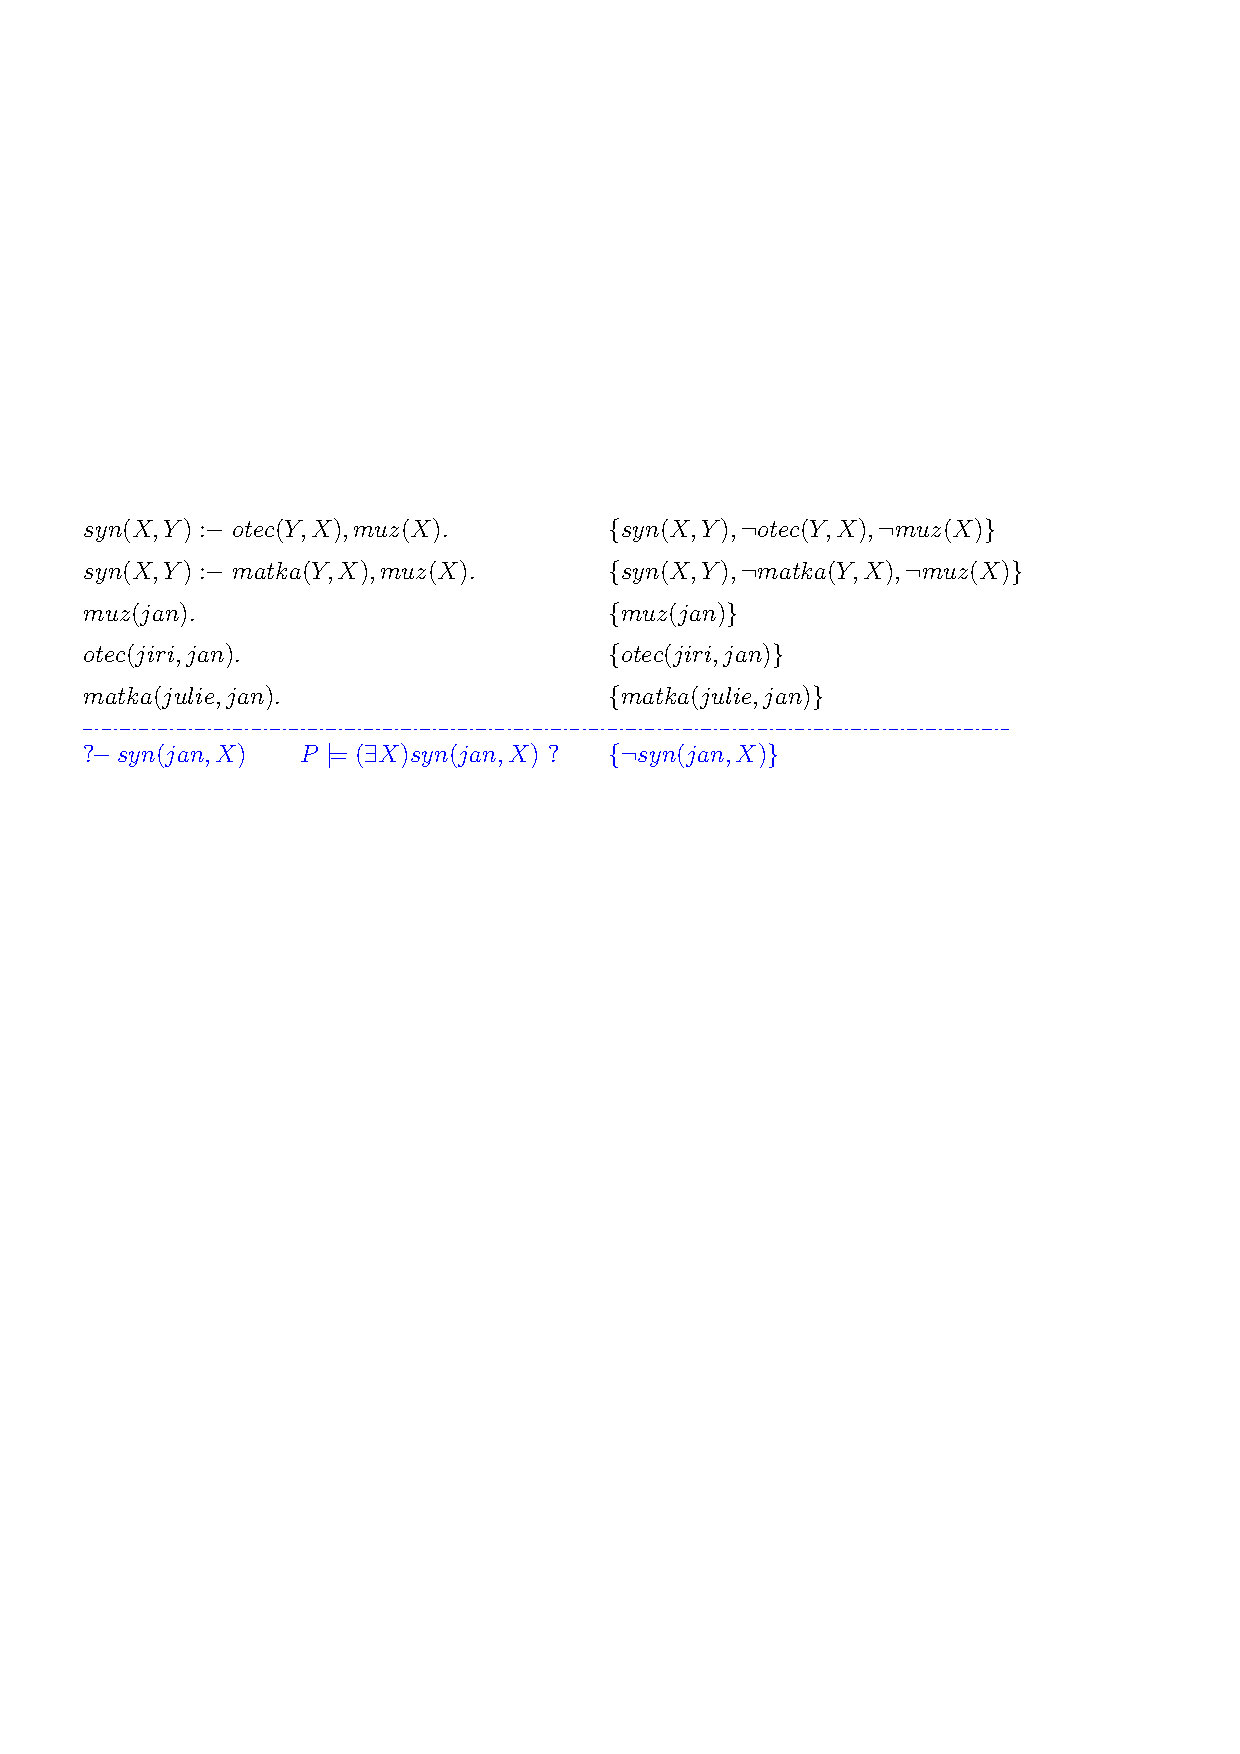
\includegraphics[scale=0.7]{files/rezolucePLprogram}}
    \bigskip
    
    {\it Zajímá nás, zda daný \myblue{existenční dotaz} vyplývá z daného programu.}%, navíc to chceme doložit \myblue{výstupní substitucí}.
    \medskip
    
    {\bf \myblue{Důsledek}}\ \ {\it Pro program $P$ a cíl $G=\{\neg A_1, \dots, \neg A_n\}$ v proměnných $X_1,\dots,X_m$
    
    \vspace{-0mm}
    \begin{enumerate}
    \item[$(1)$] $P \models (\exists X_1)\dots(\exists X_m)(A_1\mand \dots \mand A_n)$, právě když
    \smallskip
    
    \item[$(2)$] $\square$ lze odvodit LI-rezolucí z $P\cup\{G\}$ začínající (variantou) cíle $G$.
    \end{enumerate}}
    
    
    %%%%%%%%%%%%%%%%%%%%%%%%%%%%%%%%%%%%%%%%%%%%%%%%%%%%%%5
    
    \subsubsection*{LI-rezoluce nad programem}
    {\it Je-li odpověď na dotaz kladná, chceme navíc znát výstupní substituci.}
    \medskip
    
    \mdef{Výstupní substituce} $\sigma$ LI-rezoluce $\square$ z $P\cup\{G\}$ začínající $G=\{\neg A_1,\dots,\neg A_n\}$
    \smallskip
    
    je složení \myblue{mgu} v jednotlivých krocích (jen na proměnné v $G$). Platí,
    \vspace{-2mm}
    \mygreen{$$P \models (A_1 \mand \dots \mand A_n)\sigma.$$}
    
    \vspace{-2mm}
    
    \centerline{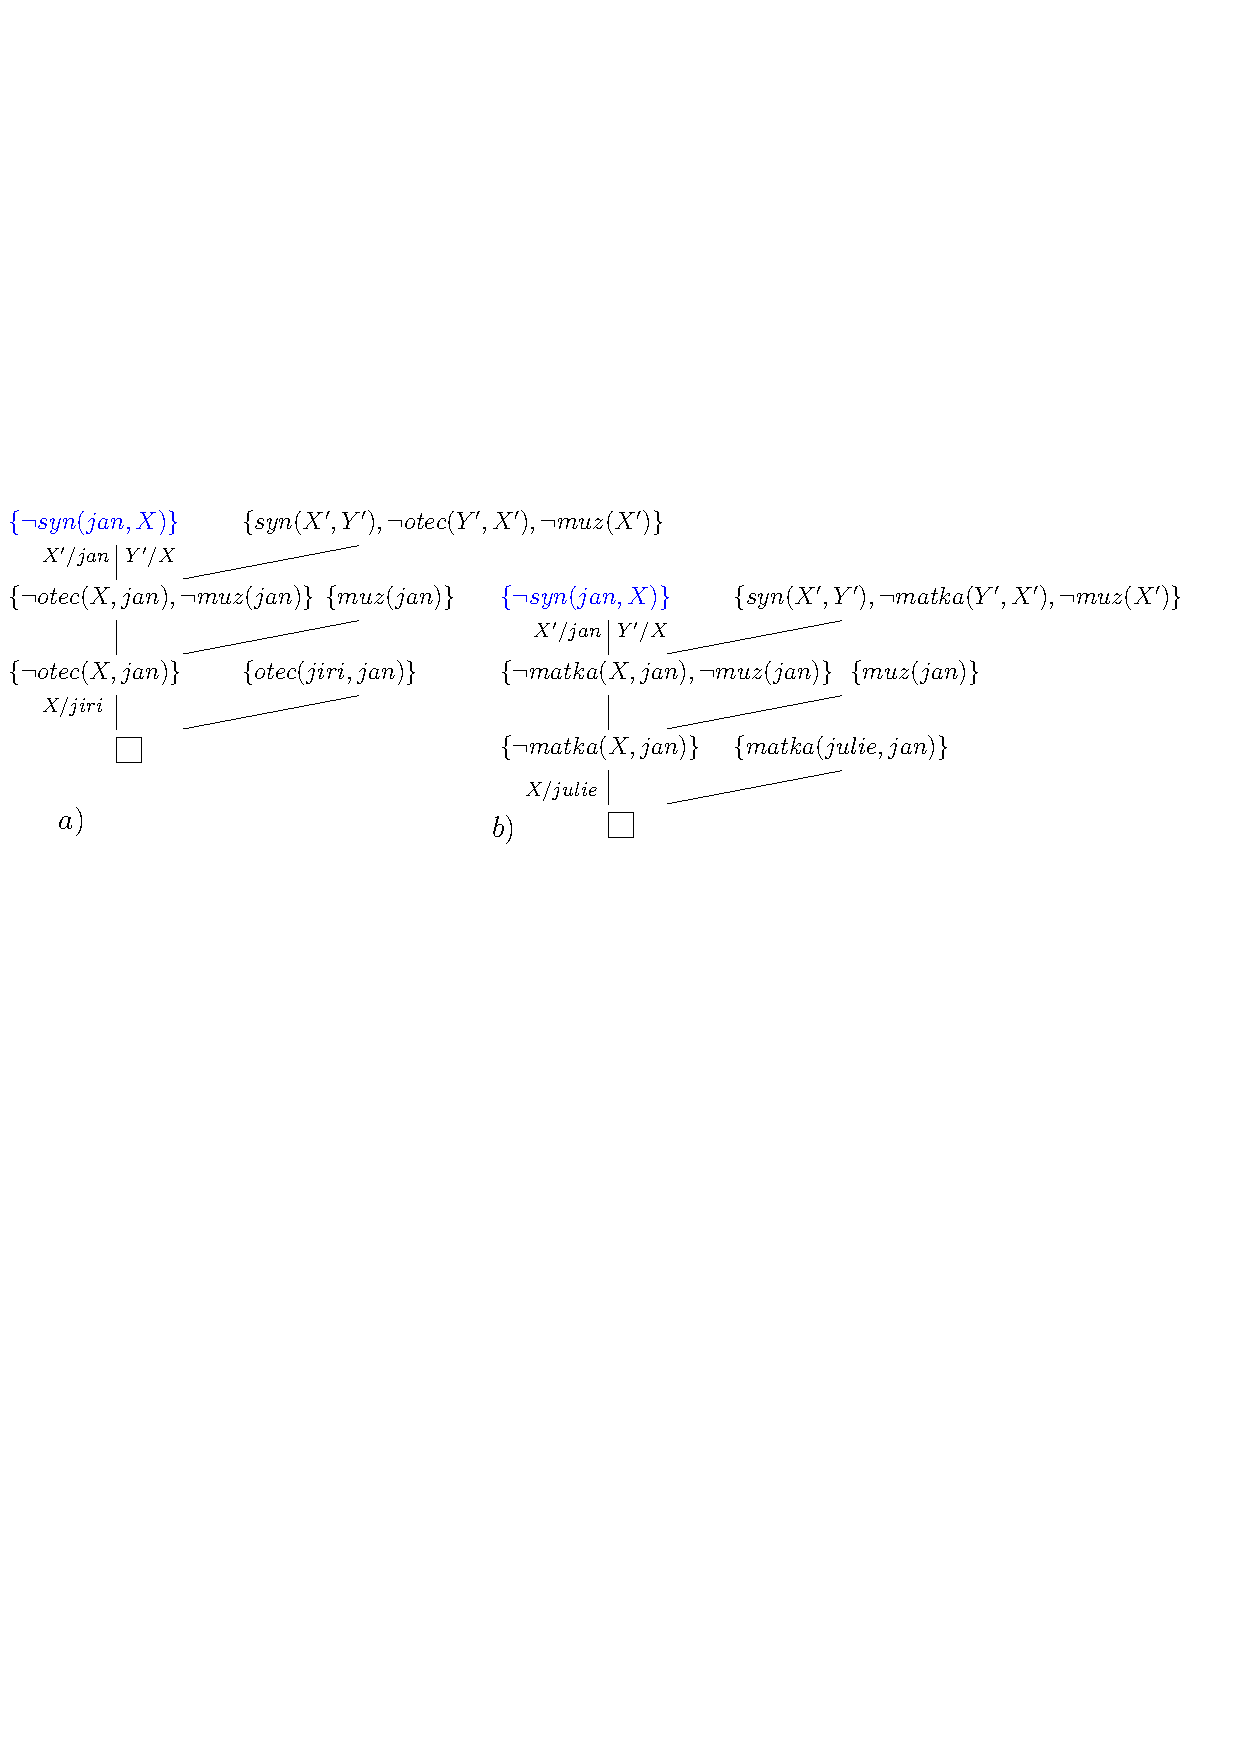
\includegraphics[scale=0.63]{files/rezolucePLprogramLI}}
    \bigskip
    
    Výstupní substituce $a)$ $X=jiri$,\ \ $b)$ $X=julie$.
    
    
% :from slides



